\section{Anforderungen}

\subsection{Personas}
Unter der Definition von Personas\footcite{persona_definition} versteht man: 
\begin{displayquote}
Personas (lat. Maske) sind Nutzermodelle, die Personen einer Zielgruppe in ihren Merkmalen charakterisieren. Sie können z. B. einem Entwicklerteam aufgrund ihrer umfangreichen Beschreibung helfen, sich in die Lage der potenziellen Nutzer zu versetzen und diese Perspektive während des gesamten Designprozesses leicht zu vertreten. Sie werden mit einem Namen, einem Gesicht, einer Funktion, einem Werdegang und einem Privatleben versehen. Personas verfügen über Ziele und Verhaltensweisen, haben Vorlieben und Erwartungen.
\end{displayquote}

Diese Personas wurden erstellt, um ein klareres Bild vermitteln zu können, welche Funktionalitäten durch den Aufgaben-Coach ermöglicht werden und wie diese Anwendung eingesetzt werden könnte.

\subsubsection{Persona 1}
\subsubsection*{Persönliches Profil}
Abirsana ist Lehrerin an der Schule Gossau und unterrichtet die Fächer Mathematik, Deutsch und Englisch.

\subsubsection*{Situation}
Um den Unterricht interessanter zu gestalten, greift Abirsana oft auf digitale Medien, wie zum Beispiel YouTube Videos, zurück. Oftmals ist jedoch das Material nicht genau auf den Schulstoff angepasst oder die Qualität lässt zu wünschen übrig. Zudem braucht sie sehr lange, um passende Videos zu finden.

\subsubsection*{Szenario}
Im Rahmen des Unterrichts soll es Abirsana möglich sein, die Aufgaben-Coach Webanwendung zu verwenden. Sie soll in der Lage sein, einzelne Fächer und Theorieinhalte ihrer Klasse zur Verfügung zu stellen. Zudem kann sie eigene Übungen erfassen, welche die Schüler direkt über die Webanwendung lösen können. Sind die Aufgaben abgegeben, kann sie die einzelnen Aufgaben anschauen und bewerten. Falls ihr auffällt, dass ein gewisser Schüler oder die ganze Klasse etwas nicht versteht, kann sie eingreifen und Wissenslücken schliessen.

\subsubsection{Persona 2}
\subsubsection*{Persönliches Profil}
Salina ist Schülerin an einer Schule. Seit längerer Zeit hat sie jedoch Mühe mit dem Schulstoff und ist nicht zufrieden mit ihrer Schulleistung.

\subsubsection*{Situation}
Salina versteht den Lernstoff oft nicht, wenn ihr Lehrer ihr etwas erklärt. Zu Hause verbringt sie dann viel Zeit im Internet, um einzelne Themen zu lernen. Sie hat aber weder die Zeit noch die Lust dazu, zu Hause nochmals die gesamte Theorie anschauen zu müssen und nach guten Videos zu suchen.

\subsubsection*{Szenario}
Nach kurzer Zeit hat Salina die Lehrer an ihrer Schule dazu überredet, die Aufgaben-Coach Plattform einzusetzen. Somit ist Salina freier im Lernen. In der Schule kann sie sich selbstständig ein Thema beibringen. Falls sie dennoch etwas nicht versteht, kann sie direkt auf eine Lehrperson zugehen, welche ihr dann das Kapitel vielleicht noch etwas genauer erklärt. \\
Zudem fällt es Salina einfacher Fragen zu stellen. Zuvor hatte sie immer das Gefühl, die ganze Klasse aufzuhalten. Nun kann sie in Ruhe ihre Fragn stellen, während die anderen Schüler selbstständig weiter lernen können. Des Weiteren verbringt sie zu Hause auch nicht mehr so viel Zeit mit dem Suchen von Videos, da sich alle benötigten Theorieinhalte auf Aufgaben-Coach befinden.

\subsubsection{Persona 3}
\subsubsection*{Persönliches Profil}
Liam ist ebenfalls Lehrer an einer Schule. Er mag es am liebsten, wenn er genau weiss, was vor sich geht. Überraschungen kann er gar nicht leiden und besonders dann nicht, wenn es sich dabei um schlechte Resultate seiner Schüler bei einer Prüfung handelt.

\subsubsection*{Situation}
Immer wieder kommt es vor, dass seine Schüler eine Prüfung schlechter abschneiden, als er sich das erhofft. Dem will er nun ein Ende setzten und sucht nach einer Lösung.

\subsubsection*{Szenario}
Um in Zukunft unangenehme Überraschungen wie diese zu vermeiden, will er eine Möglichkeit haben, genauere Details über den aktuellen Wissensstand seiner Schüler zu sammeln. Um dieses Ziel zu erreichen, möchte er keinen grossen Mehraufwand auf sich nehmen und will den Unterricht so wie bisher weiterführen.


\subsection{Funktionale Anforderungen}

\subsubsection{Use Case Diagramm}
In der Abbildung \ref{uc_diagram} ist das Use Case Diagramm abgebildet. Dieses Diagramm soll die Abhängigkeiten zwischen Aktoren, den einzelnen Use Cases und externen Systemen visualisieren.

\begin{minipage}{\textwidth}

\begin{figure}[H]
	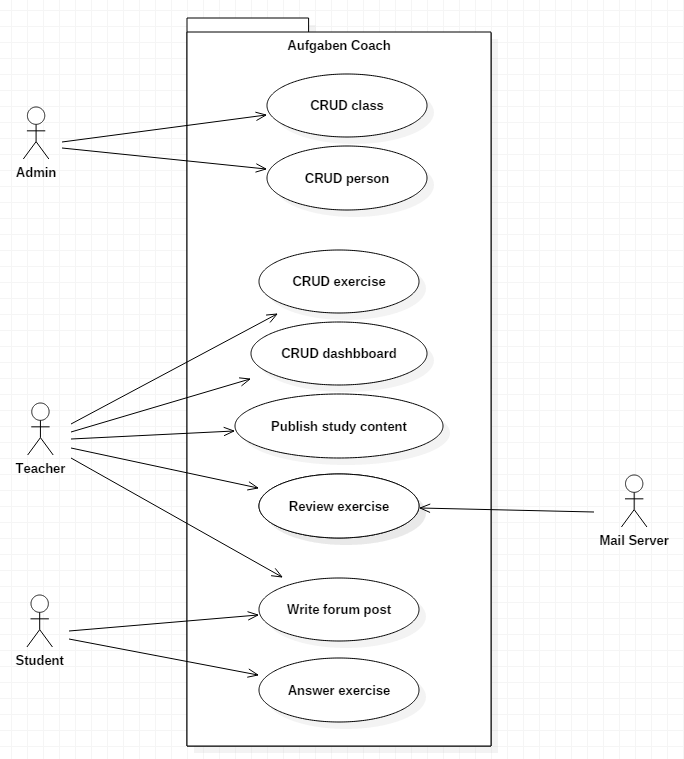
\includegraphics[width=\textwidth, height=\textheight, keepaspectratio]{images/UseCaseDiagramm.png}
	\caption{Use Case Diagramm}
	\label{uc_diagram}
\end{figure}

\end{minipage}

\newpage

\subsubsection{Aktoren}
Die Aktoren, welche mit der Anwendung interagieren, sind in der Tabelle \ref{aktoren} beschrieben. \\

\begin{table}[H]
	\centering
	\begin{tabu} to 0.9\textwidth {l X}
	\toprule
	Aktor & Beschreibung \\ 
	\midrule
	Administrator & Der Administrator ist für die Verwaltung der Klassen, Lehrer und Schüler zuständig. Er kann Klassen erstellen sowie Lehrpersonen und Schüler diesen Klassen zuweisen. \\
	\midrule
	Lehrer & Der Lehrer verwaltet die ihm zugewiesenen Klassen. Er kann Fächer für seine Klassen freischalten sowie Aufgaben erstellen und diese der Klasse zuweisen. Zusätzlich kann er Statistiken einsehen, die ihn über den aktuellen Wissensstand seiner Klasse informieren. \\
	\midrule
	Schüler & Die Schüler haben Zugriff auf freigeschaltete Lerninhalte und können diese anschauen. Falls Fragen auftreten, können diese im aufgaben-spezifischen Forum gestellt werden. Zusätzlich können Aufgaben gelöst werden. \\
	\midrule
	Mail Server & Der Mail Server dient dem Versenden von Nachrichten, falls zum Beispiel eine Lehrperson ein Feedback an einen Lernenden schicken möchte. \\
	\bottomrule
	\end{tabu}
	\captionof{table}{Aktoren}
	\label{aktoren}
\end{table}


\subsubsection{Use Case Beschreibung}
Nachfolgend werden die einzelnen Use Cases stichwortartig beschrieben. 
\subsubsection*{CRUD person}

\begin{itemize}
	\item Hauptszenario:
	\begin{itemize}
		\item Der Administrator kann neue Benutzer erstellen. Diese können entweder die Rolle ''Schüler'' oder ''Lehrer'' haben.
	\end{itemize}
	\item Alternatives Szenario:
	\begin{itemize}
		\item Der Administrator entfernt einen Benutzer aus dem System.
		\item Der Administrator ändert Angaben eines Benutzers.
	\end{itemize}
\end{itemize}

\newpage

\subsubsection*{CRUD class}

\begin{itemize}
	\item Hauptszenario:
	\begin{itemize}
		\item Der Administrator erstellt eine neue Klasse, welcher Lehrpersonen und Schüler zugewiesen werden können.
	\end{itemize}
	\item Alternatives Szenario:
	\begin{itemize}
		\item Nach Ablauf eines Schuljahres kann der Administrator Klassen aus dem System entfernen.
		\item Der Administrator kann einzelne Schüler aus einer Klasse entfernen und diese einer anderen Klasse zuweisen.
	\end{itemize}
\end{itemize}


\subsubsection*{CRUD exercise}
\begin{itemize}
	\item Hauptszenario:
	\begin{itemize}
		\item Der Lehrer kann neue Aufgaben erstellen und diese einem Thema zuweisen. Pro Aufgabe gibt es mehrere Fragen, welche wiederum mehrere Hilfestellungen enthalten können. Für jede Frage kann auch eine maximale Punktzahl angegeben werden. 
	\end{itemize}
	\item Alternatives Szenario:
	\begin{itemize}
		\item Der Lehrer passt einzelne Fragen oder Hilfestellungen an oder fügt neue Fragen einer Aufgabe hinzu.
	\end{itemize}
\end{itemize}



\subsubsection*{CRUD dashboard}
\begin{itemize}
	\item Hauptszenario:
	\begin{itemize}
		\item Der Lehrer passt den Wochenplan einer Klasse an und fügt neue Aufgaben hinzu.
	\end{itemize}
	\item Alternatives Szenario:
	\begin{itemize}
		\item Der Lehrer verschiebt den Abgabetermin einer Aufgabe auf einen anderen Tag.
	\end{itemize}
\end{itemize}



\subsubsection*{Publish study content}
\begin{itemize}
	\item Hauptszenario:
	\begin{itemize}
		\item Der Lehrer kann Fächer für einzelne Klassen freischalten.
	\end{itemize}
	\item Alternatives Szenario:
	\begin{itemize}
		\item Freigeschaltene Fächer können wieder entfernt werden.
	\end{itemize}
\end{itemize}



\subsubsection*{View statistics}
\begin{itemize}
	\item Hauptszenario:
	\begin{itemize}
		\item Der Lehrer hat Einsicht in die Statistiken einzelner Klassen oder Schüler.
	\end{itemize}
\end{itemize}


\subsubsection*{Write forum post}
\begin{itemize}
	\item Hauptszenario:
	\begin{itemize}
		\item Treten beim Lösen von Aufgaben Unklarheiten auf, kann ein Schüler eine entsprechende Frage direkt im aufgabenspezifischen Forum stellen.
	\end{itemize}
	\item Alternatives Szenario:
	\begin{itemize}
		\item Ein Schüler sieht eine Frage im Forum, zu welcher er die Lösung weiss. Er kann auf den Beitrag seines Schulkameraden antworten und ihm so helfen.
	\end{itemize}
\end{itemize}


\subsubsection*{Review exercise}
\begin{itemize}
	\item Hauptszenario:
	\begin{itemize}
		\item Der Lehrer hat die Möglichkeit, gelöste Aufgaben der Schüler zu korrigieren und zu bewerten. Nach der Bewertung kann die Abgabe akzeptiert werden.
	\end{itemize}
	\item Alternatives Szenario:
	\begin{itemize}
		\item Der Lehrer stellt beim Korrigieren der Abgabe zu viele Fehler fest und entscheidet sich die Abgabe an den Schüler zurückzuweisen. Er kann für den Schüler ein Feedback schreiben, welches per Mail versendet wird.
	\end{itemize}
\end{itemize}


\subsubsection*{Answer exercise}
\begin{itemize}
	\item Hauptszenario:
	\begin{itemize}
		\item Der Schüler kann die Aufgaben von freigegebenen Fächern lösen. Sind alle Fragen beantwortet, kann die Übung abgegeben und vom Lehrer korrigiert werden.
	\end{itemize}
	\item Alternatives Szenario:
	\begin{itemize}
		\item Falls der Lehrer die Übung eines Schülers zurückweist, kann dieser die Fragen nochmals überarbeiten.
	\end{itemize}
\end{itemize}

\newpage

\subsection{Nicht Funktionale Anforderungen}
\label{chapter_nfr}
Bei der Erstellung der einzelnen \gls{nfr} wird auf FURPS zurückgegriffen. FURPS ist ein Akronym für Functionality, Usability, Reliability, Performance und Supportability. Dieses Modell wurde im Jahre 1992 von HP entwickelt und dient zur Priorisierung der Software Requirements\footcite{furps_description}. \\

\begin{table}[h]
	\centering
	\begin{tabu} to 0.9\textwidth {l l X}
	\toprule
	FURPS & Titel & Beschreibung \\ 
	\midrule
	Functionality & Reusability & Die Anwendung soll so entwickelt werden, dass sie an mehreren Schulen eingesetzt werden kann. \\
	& 	Security & Die Rechte der einzelnen Benutzer sind eingeschränkt. Niemand hat per Default Zugriff auf alles. \\
	&  & Die Webseite ist nur über HTTPS erreichbar. \\
	\midrule
	Usability & Responsiveness & Für Schüler soll die Applikation sowohl auf Tablets wie auch auf Mobile Phones verfügbar sein. \\
	\midrule
	Reliability & Availability & Die Anwendung ist stabil und stürzt nicht ab. \\
	& Fault Tolerance & Die Anwendung soll auch bei unerlaubten Anfragen weiterhin verfügbar sein und die korrekten Ergebnisse liefern. \\
	\midrule
	Performance & Availability & Die Anwendung soll ohne abzustürzen von 300 Benutzern zeitgleich verwendet werden können. \\
	 & Response Time & Wechselt der Benutzer zwischen einzelnen Seiten, soll die neue Seite in maximal einer Sekunde geladen werden.\\
	\midrule
	Supportability & Maintainability & Die Applikation soll so gebaut werden, dass sie auch in Zukunft gewartet und ausgebaut werden kann. \\
	 & Installability & Die Applikation wird so gebaut, dass sie innerhalb einer Stunde auf einem neuen System installiert werden kann. \\
	\bottomrule
	\end{tabu}
	\captionof{table}{Non Functional Requirements}
	\label{nfr}
\end{table}


\newpage